\section{Implementation and Experiment Settings} \label{sec_experiment}
This section presents a comprehensive evaluation of our proposed dual-branch framework. We organize the experiments around three research questions (RQs), describe the datasets and experimental setup, and then report results on in-dataset, cross-dataset, and adversarial robustness evaluations. Our goal is to rigorously assess accuracy, generalization, and resilience. 

\begin{table*}[ht]
\centering
\caption{Summary of datasets used in the experiments.}
\label{tab:dataset}
\begin{tabular}{lccccc}
\toprule
\textbf{Dataset} & \textbf{Year} & \textbf{Samples} & \textbf{Features} & \textbf{Classes} & \textbf{Used} \\
\midrule
IoTDIAD & 2023 & $\sim$1.2M & 35 & 9 (1 benign + 8 attacks) & 180k \\
ACI IoT & 2023 & $\sim$25M & 42 & 16 (1 benign + 15 attacks) & 320k \\
\bottomrule
\end{tabular}
\end{table*}

\subsection{Research Questions}
To evaluate the performance of our approach, we define the following research questions:
\begin{itemize}
    \item \textbf{RQ1: Defense Effectiveness.} Does P4P maintain higher accuracy and achieve a lower Attack Success Rate (ASR) than existing defense methods under Byzantine and Backdoor attack scenarios?
    
    \item \textbf{RQ2: Non-IID Robustness.} Can P4P accurately detect malicious updates without confusing them with Non-IID induced drifts, and perform better than baseline approaches?
    
    \item \textbf{RQ3: Component Contribution.} What is the contribution of each individual component of the P4P framework (i.e., Probe Vector, L2-norm Filtering, and Temporal Scoring) to its overall defense performance?
    
    \item \textbf{RQ4: Overhead and Practicality.} Does P4P achieve low computational and communication overhead, making it practical for deployment in IDS or edge computing environments?
\end{itemize}

Rationale for RQ Selection. Our research questions are designed to systematically evaluate the defensive effectiveness, internal component contributions, and practical viability of the P4P framework under realistic FL conditions.
RQ1 (Defense Effectiveness) examines whether P4P can maintain model accuracy and effectively reduce the Attack Success Rate (ASR) compared to existing defense methods under Byzantine and Backdoor attack scenarios. This question focuses on the core hypothesis that P4P’s design provides stronger resilience against adversarial manipulation without sacrificing global performance.
RQ2 (Non-IID Robustness) investigates P4P’s capability to accurately distinguish malicious updates from legitimate Non-IID deviations. Since Non-IID data distributions are inevitable in real-world federated systems, this RQ evaluates whether P4P avoids false detections while maintaining robustness as the degree of data heterogeneity increases.
RQ3 (Component Contribution) is designed to validate our design choices by quantifying the individual impact of each key module. By conducting an ablation study, we assess how the Probe Vector, L2-norm Filtering, and Temporal Scoring each contribute to the framework's overall resilience, ensuring that the multi-layer design is both effective and necessary.
RQ4 (Overhead and Practicality) assesses whether P4P achieves low computational and communication overhead, ensuring it is lightweight enough for deployment in Intrusion Detection Systems (IDS) or edge computing environments. This RQ emphasizes the framework’s scalability and feasibility beyond controlled research settings.
We intentionally focus on these aspects effectiveness, robustness, component contribution, and practicality as they represent the essential properties of a deployable and trustworthy federated defense mechanism. Other factors such as interpretability or hyperparameter sensitivity, while relevant, are considered secondary at this stage and are left for future exploration.

\begin{table}[t]
\centering
\caption{Model configuration (MLP).}
\label{tab:model_config}
\begin{tabular}{lccc}
\toprule
Model & Hidden Layers & Units & Activation\\
\midrule
MLP (ours) & 2 FC + Output & [128, 64] & ReLU \\
\bottomrule
\end{tabular}
\end{table}

\subsection{Experimental Setup}
\subsubsection{Datasets}

Table~\ref{tab:dataset} summarizes the key characteristics of the datasets used in our experiments.

We evaluate our method on publicly available flow-based IoT intrusion detection datasets released by the Canadian Institute for Cybersecurity (CIC):

\begin{itemize}
    \item \textbf{IoTDIAD Dataset (2024)}~\cite{IoTDIAD2024}: 
    A comprehensive IoT traffic dataset that includes both benign and multiple attack scenarios 
    (e.g., DDoS, DoS, scanning, brute force, and injection attacks). 
    The raw dataset contains millions of flow-based records captured from diverse IoT devices. 
    For computational efficiency and balanced evaluation, we randomly selected 
    approximately 180,000 representative flow records (20,000 per class), 
    maintaining the original benign–malicious ratio and temporal characteristics.

    \item \textbf{ACI IoT Network Traffic Dataset (2023)}~\cite{ACI2023}: 
    Another realistic IoT dataset combining smart-home and industrial IoT environments. 
    It encompasses over 25 million packets labeled into benign and 15 attack categories. 
    We extracted a stratified subset of 320,000 samples (20,000 per class) 
    to mitigate label imbalance and ensure reproducibility under federated non-IID settings.
\end{itemize}

\subsubsection{Model Architecture}

Table~\ref{tab:model_config} presents the configuration of the MLP model used in all experiments.

For all experiments, we employ a lightweight multi-layer perceptron (MLP) 
designed for flow-based intrusion detection. 
The model comprises two hidden fully connected layers with 128 and 64 neurons, respectively,
each followed by ReLU activation and dropout ($p=0.2$) to prevent overfitting. 
A final linear layer maps the latent representation to the number of attack classes. 
This compact architecture offers an excellent balance between detection accuracy 
and computational efficiency, making it suitable for deployment 
in federated and edge-based IDS environments.

\subsubsection{Preprocessing and Labeling}
\label{sec:preprocessing}

For the \textbf{IoTDIAD} dataset, preprocessing begins with removing privacy-sensitive network identifiers, including \texttt{Flow ID, IPs, ports, and Timestamp}. The multi-class \texttt{Label} is integer-encoded (0-6), and numerical stability is improved by replacing infinite and NaN values. All numeric features are subsequently standardized to a zero mean and unit variance using \textit{StandardScaler}. Finally, an ANOVA F-test-based feature selection (\textit{SelectKBest}) is applied to retain the top 30 most discriminative features.

The pipeline for the \textbf{ACI-IoT} dataset is distinct. Multiple source files are first merged, and labels are mapped to binary integers (\texttt{Benign}: 0, \texttt{Attack}: 1). To counter a severe class imbalance, we perform \textit{undersampling} on the majority 'Attack' class. In contrast to standardization, all features are normalized to a [0, 1] range via \textit{MinMaxScaler}. No feature selection is applied to this dataset; all original features are retained.

\label{sec:training-config}

\begin{table}[h!]
\caption{Hyperparameters and Experimental Configuration}
\centering
\begin{tabular}{ll}
\toprule
\textbf{Parameter} & \textbf{Value} \\
\midrule
Federated algorithms & FedAvg \\
Number of clients & 20 \\
Rounds & 15 \\
Local epochs per client & 5 \\
Batch size & 32 \\
Learning rate & 0.01 \\
Malicious client fraction & 30\% \\
Data partition type & Non-IID ($\alpha \in \{0.1, 0.5, 1.0\}$) \\
Random seed & 42 \\
Platform & P100 GPU (Kaggle) \\
Framework / Libraries & PyTorch, CUDA \\
\bottomrule
\end{tabular}
\label{tab:hyperparameters}
\end{table}

\subsection{Training Configuration}

All experiments are conducted under a standard Federated Averaging (FedAvg) framework. The key hyperparameters and experimental settings are summarized in Table~\ref{tab:hyperparameters}. The system comprises 20 clients and 15 rounds of global communication. In each round, every client performs 5 local epochs of training with a mini-batch size of 32 and a learning rate of 0.01. The local optimizer utilizes Stochastic Gradient Descent (SGD), and model parameters are aggregated on the central server according to the FedAvg algorithm to update the global model.

In this setup, 30\% of the clients are designated as malicious. Data are partitioned among clients in a non-identically and independently distributed (Non-IID) manner. This is achieved using a Dirichlet distribution with concentration parameters $\alpha \in \{0.1, 0.5, 1.0\}$ to simulate varying degrees of data heterogeneity.

All defense mechanisms, including No\_Def, FedMP, Recess, and our proposed P4P, are applied during the server aggregation phase after receiving local updates from clients. To ensure a fair comparison, each defense mechanism uses identical training hyperparameters, differing only in their aggregation logic and attack detection strategies.

Training and evaluation are performed on a P100 GPU on the Kaggle platform, using PyTorch 2.0 and CUDA 12. The reproducibility of the experiments is ensured by setting a fixed random seed of 42.

\subsubsection{Baselines}

We compare our proposed \textit{P4P} defense against three baseline aggregation strategies in the FL setting:

\begin{itemize}
    \item \textbf{No\_Def:} the standard FedAvg aggregation without any defense mechanism. This serves as the vulnerable baseline to quantify the effect of each attack.
 
    \item \textbf{FedMP:} a model-parameter filtering method that removes suspicious updates based on their deviation from the median client gradient norm. It is effective against extreme outliers, but may over-prune benign updates under non-IID distributions.
    \item \textbf{Recess:} a reputation-based approach that gradually decays the influence of clients identified as anomalous over multiple rounds, improving long-term stability but adapting slowly to abrupt attacks.
       \item \textbf{P4P (ours):} our proposed defense, which dynamically weights client contributions using a Median Absolute Deviation (MAD)-based consistency score combined with an adaptive decay factor. P4P aims to maintain high accuracy, while suppressing both additive and multiplicative poisoning behaviors.
\end{itemize}

\subsubsection{Adversarial Attack Simulation}

To comprehensively assess robustness, we simulate six representative poisoning attacks targeting the federated aggregation process:

\begin{itemize}
    \item \textbf{LIE attack} ~\cite{baruch2019little}: malicious clients submit exaggerated gradients to bias the global update direction.
    \item \textbf{Sign-flip attack}~\cite{fung2020limit}: attackers invert gradient signs to maximize divergence and destabilize convergence.
    \item \textbf{Scaling attack}~\cite{blanchard2017machine}: gradients are multiplied by a large scalar to dominate the aggregation.
    \item \textbf{Gaussian attack}~\cite{bhagoji2019analyzing}: random Gaussian noise is added to the model updates to introduce stochastic corruption.
    \item \textbf{Label-flip attack}~\cite{xie2019dba}: adversaries intentionally invert labels on their local data to poison the learning objective.
    \item \textbf{Backdoor attack}~\cite{bagdasaryan2020backdoor1}: a fixed input trigger (e.g., \texttt{Flow Duration = 99999}) is inserted into local data, forcing the model to misclassify target samples.
\end{itemize}

\begin{figure*}[h!]
    \centering
    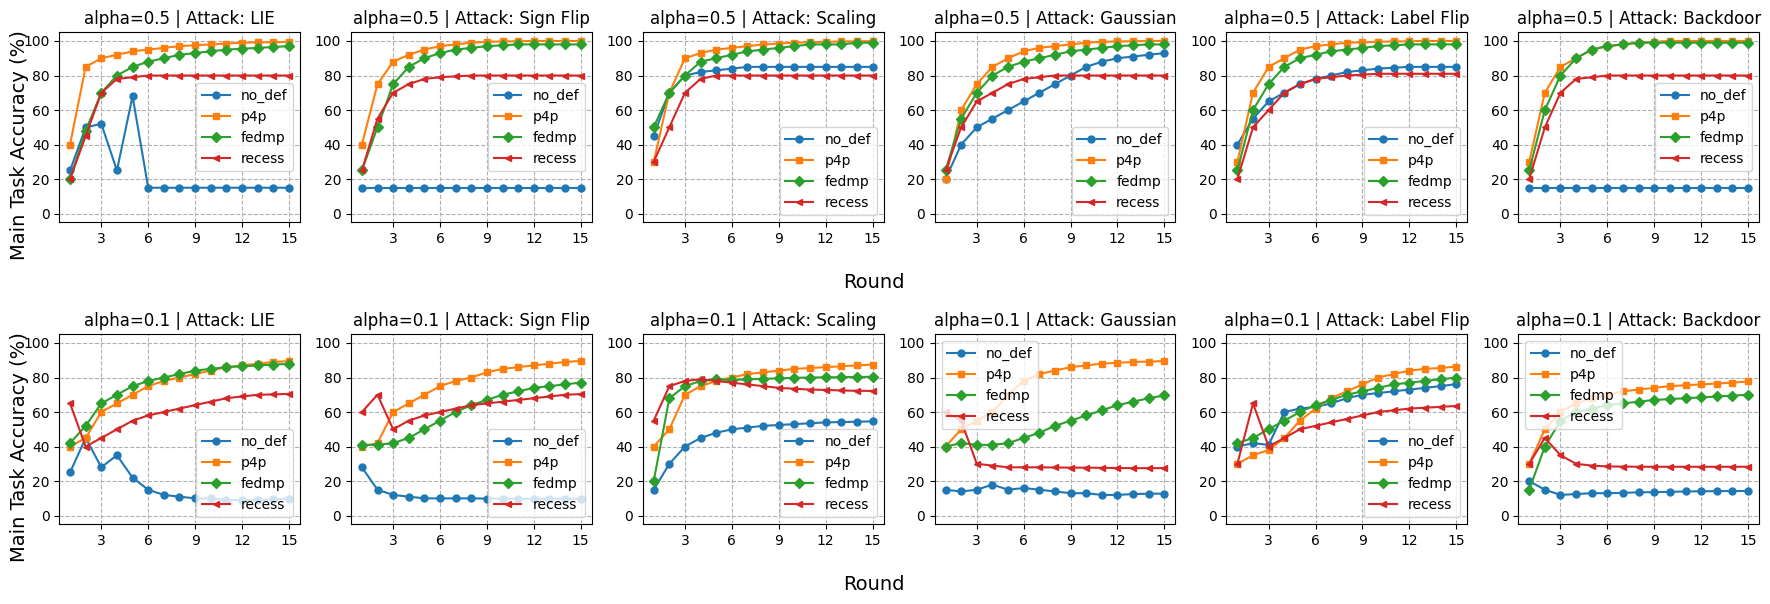
\includegraphics[width=0.99\linewidth]{images/RQ1_combined.png}
    \caption{Performance comparison across poisoning attacks on IoTDIAD dataset.}
    \label{fig:accuracy_comparison1}
\end{figure*}

Each attack is applied to 30\% of the clients (malicious fraction = 0.3) under a non-IID data partitioning scheme. For each defense, we record accuracy, macro-F1, and attack success rate (ASR) across all rounds and report the mean and standard deviation over three random seeds. This setup enables a systematic evaluation of both the effectiveness and stability of each aggregation method under diverse adversarial conditions.
